\documentclass{article}

\usepackage{booktabs}
\usepackage{tabularx}
\usepackage{graphicx}
\usepackage{float}
\usepackage{hyperref}
\hypersetup{
	colorlinks,
	citecolor=blue,
	filecolor=black,
	linkcolor=red,
	urlcolor=blue
}

\title{User Guide\\\progname}

\author{\authname}
\date{\today}

%% Comments

\usepackage{color}

\newif\ifcomments\commentstrue %displays comments
%\newif\ifcomments\commentsfalse %so that comments do not display

\ifcomments
\newcommand{\authornote}[3]{\textcolor{#1}{[#3 ---#2]}}
\newcommand{\todo}[1]{\textcolor{red}{[TODO: #1]}}
\else
\newcommand{\authornote}[3]{}
\newcommand{\todo}[1]{}
\fi

\newcommand{\wss}[1]{\authornote{blue}{SS}{#1}} 
\newcommand{\plt}[1]{\authornote{magenta}{TPLT}{#1}} %For explanation of the template
\newcommand{\an}[1]{\authornote{cyan}{Author}{#1}}

%% Common Parts

\newcommand{\progname}{Software Engineering} % PUT YOUR PROGRAM NAME HERE
\newcommand{\authname}{Team 16, Durum Wheat Semolina
	\\ Alexander Moica
	\\ Yasmine Jolly
	\\ Jeffrey Wang
	\\ Jack Theriault
	\\ Catherine Chen
	\\ Justina Srebrnjak } % AUTHOR NAMES                 

\usepackage{hyperref}
    \hypersetup{colorlinks=true, linkcolor=blue, citecolor=blue, filecolor=blue,
                urlcolor=blue, unicode=false}
    \urlstyle{same}
                                


\begin{document}

\begin{table}[hp]
\caption{Revision History} \label{TblRevisionHistory}
\begin{tabularx}{\textwidth}{llX}
\toprule
\textbf{Date} & \textbf{Developer(s)} & \textbf{Change}\\
\midrule
April 03, 2023 & All & Initial Document\\
\bottomrule
\end{tabularx}
\end{table}

\newpage

\maketitle
\newpage
\tableofcontents
\listoffigures
\newpage

\section{Symbols, Abbreviations and Acronyms}

\renewcommand{\arraystretch}{1.2}
\begin{tabular}{l l} 
	\toprule		
	\textbf{symbol} & \textbf{description}\\
	\midrule 
	BMI & Body Mass Index\\
	Ctrl & Control keyboard key\\
	\progname & Explanation of program name\\
	\bottomrule
\end{tabular}\\

\section{Introduction}

Utrition is a local web application that allows users to track their past meals, calories, and nutritional data in order to reach their health goals. This user guide lays out the steps needed for installing and launching Utrition. In addition, commonly performed tasks are outlined for users to easily refer to when using the application.

\section{Installation}
\subsection{Prerequisites}
Prerequisites for running Utrition are as follows.
\begin{itemize}
	\item macOS or Windows operating system
	\item Google Chrome as default web browser
	\item An internet connection
\end{itemize}

\subsection{Instructions}
The commands specified are targeted towards macOS operating systems. If the user is installing on Windows, equivalent commands are available.

\begin{enumerate}
	\item Create a new, easily-accessible folder for Utrition to be installed under. This folder will be used when launching the application.
	\item Open a terminal inside the newly created folder.
	\item Run the command ``git clone https://github.com/jeff-rey-wang/utrition.git" to download Utrition on to the device.
	\item Run the command ``cd utrition/src/utrition" to navigate to the Utrition code folder.
	\item Install all dependent packages by running ``pip install numpy tensorflow pillow flask plotly dash kaleido".
	\subitem If ``pip" is not installed, please follow the guide \href{https://pip.pypa.io/en/stable/installation/}{here}.
	\item Run the command ``node -v" in either terminal to ensure Node JS is installed. If there is no version returned, install Node JS by following the guide \href{https://nodejs.org/en/download}{here}.
	\item Run the command ``npm install react-scripts" in one terminal.
\end{enumerate}

\section{Launch Application Instructions}
Utrition is run from the command line interface. The user will need to open two terminals inside the Utrition application folder, specifically under ``src/utrition". In one terminal, the user will run ``\textbf{npm start}" which will allow the front-end user interface to be displayed and connects the front-end interface to the user’s local server (http://localhost:3000). In the second terminal, the user will run ``\textbf{npm run start-backend}" to create an unseen back-end interface on the user’s local server (http://localhost:5000). When both interfaces are set up, a web browser will automatically open to the home page of Utrition which is shown below. Once the user is on the home page, the application is ready for usage.

\begin{figure}[H]
	\centering
	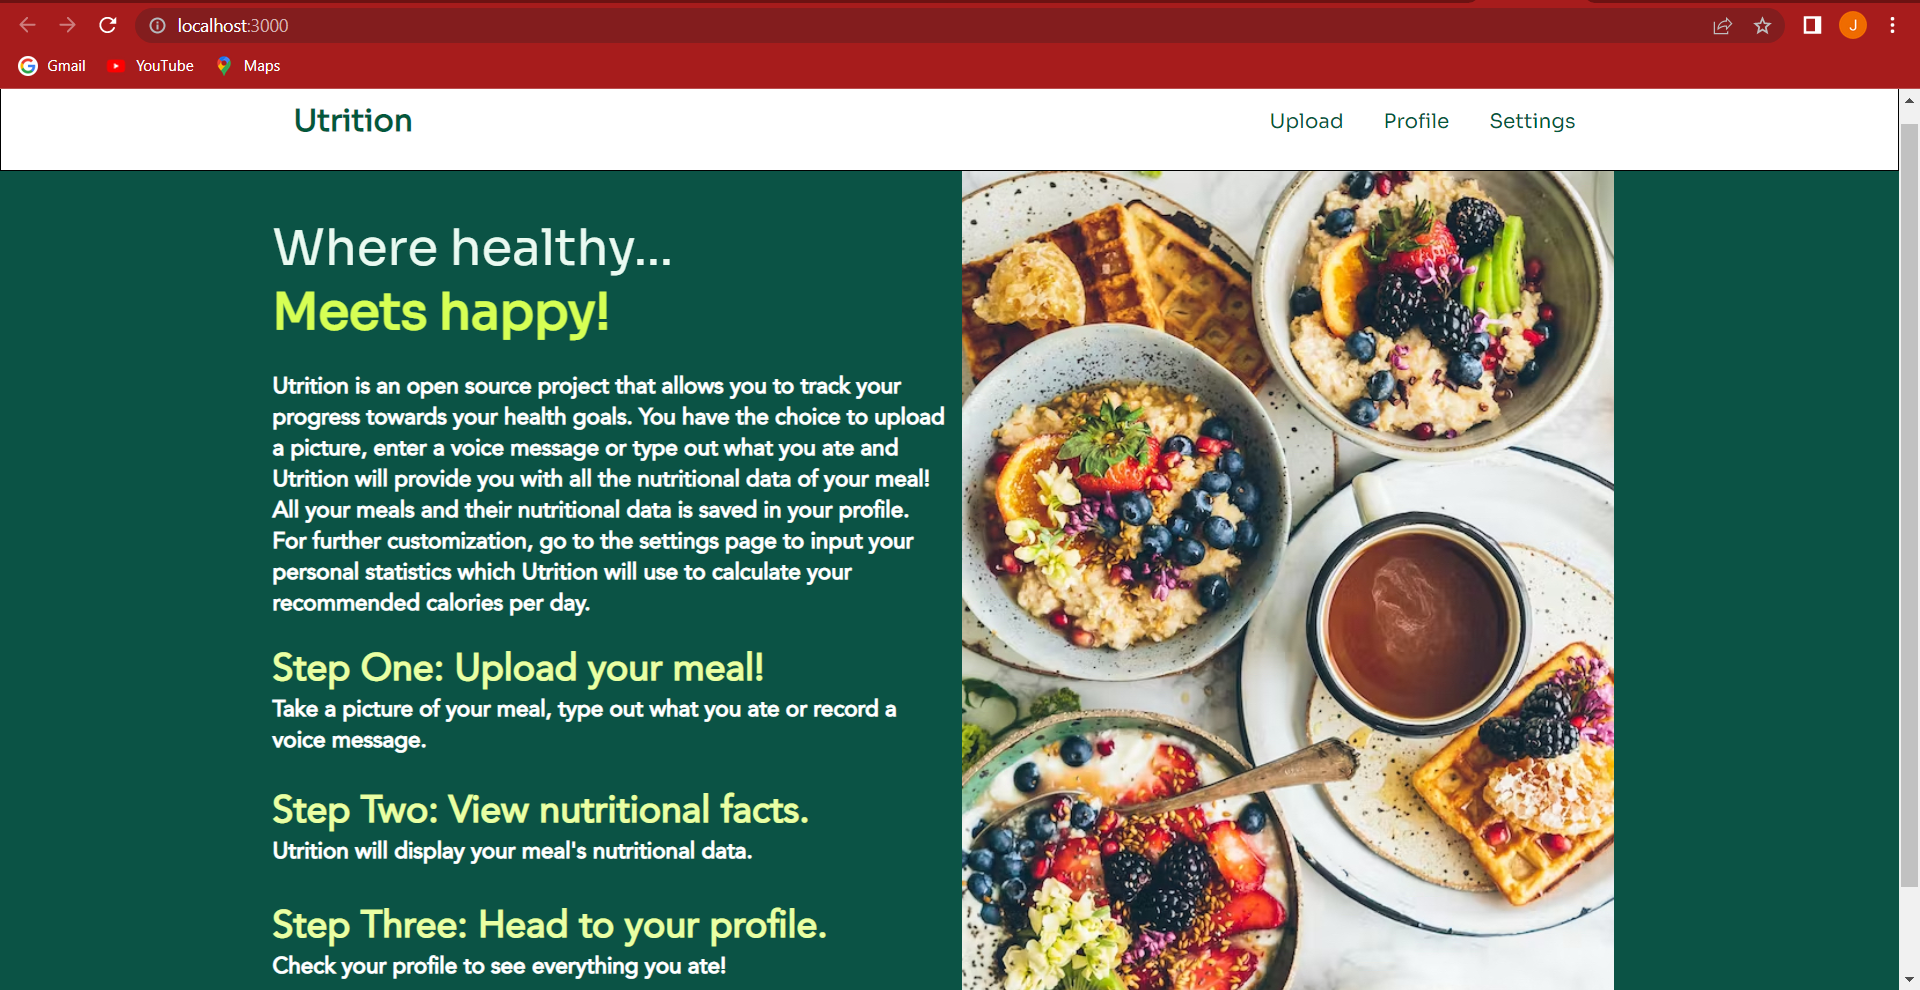
\includegraphics[scale=0.30]{homepage.png}
	\caption{Home Page of Utrition}
\end{figure}

\section{Closing Application Instructions}
Once the user has finished using Utrition, the following instructions will close the application. In both terminals used to start the application, the user should press the keyboard buttons Ctrl+C. Once this has been done in both terminals, Utrition has been shut off successfully.

\section{General Usage Tasks}
This section details the most commonly executed user functions when using Utrition. Steps for each task are shown below.
\subsection{Logging a Food Item}
When a user wishes to upload a food item they have consumed to the application, they must navigate to the ``Upload" page by clicking the ``Upload" text found in the navigation bar at the top of every page. From there, the user is brought to the ``Upload" page where they have the option to upload their food in one of three different ways. Each option is further explained in the following sections.
\subsubsection{Text Upload}
Once on the ``Upload" page, users must select the text upload button as shown in Figure 2. A text box will appear where the user can type in their food input.
\begin{figure}[H]
	\centering
	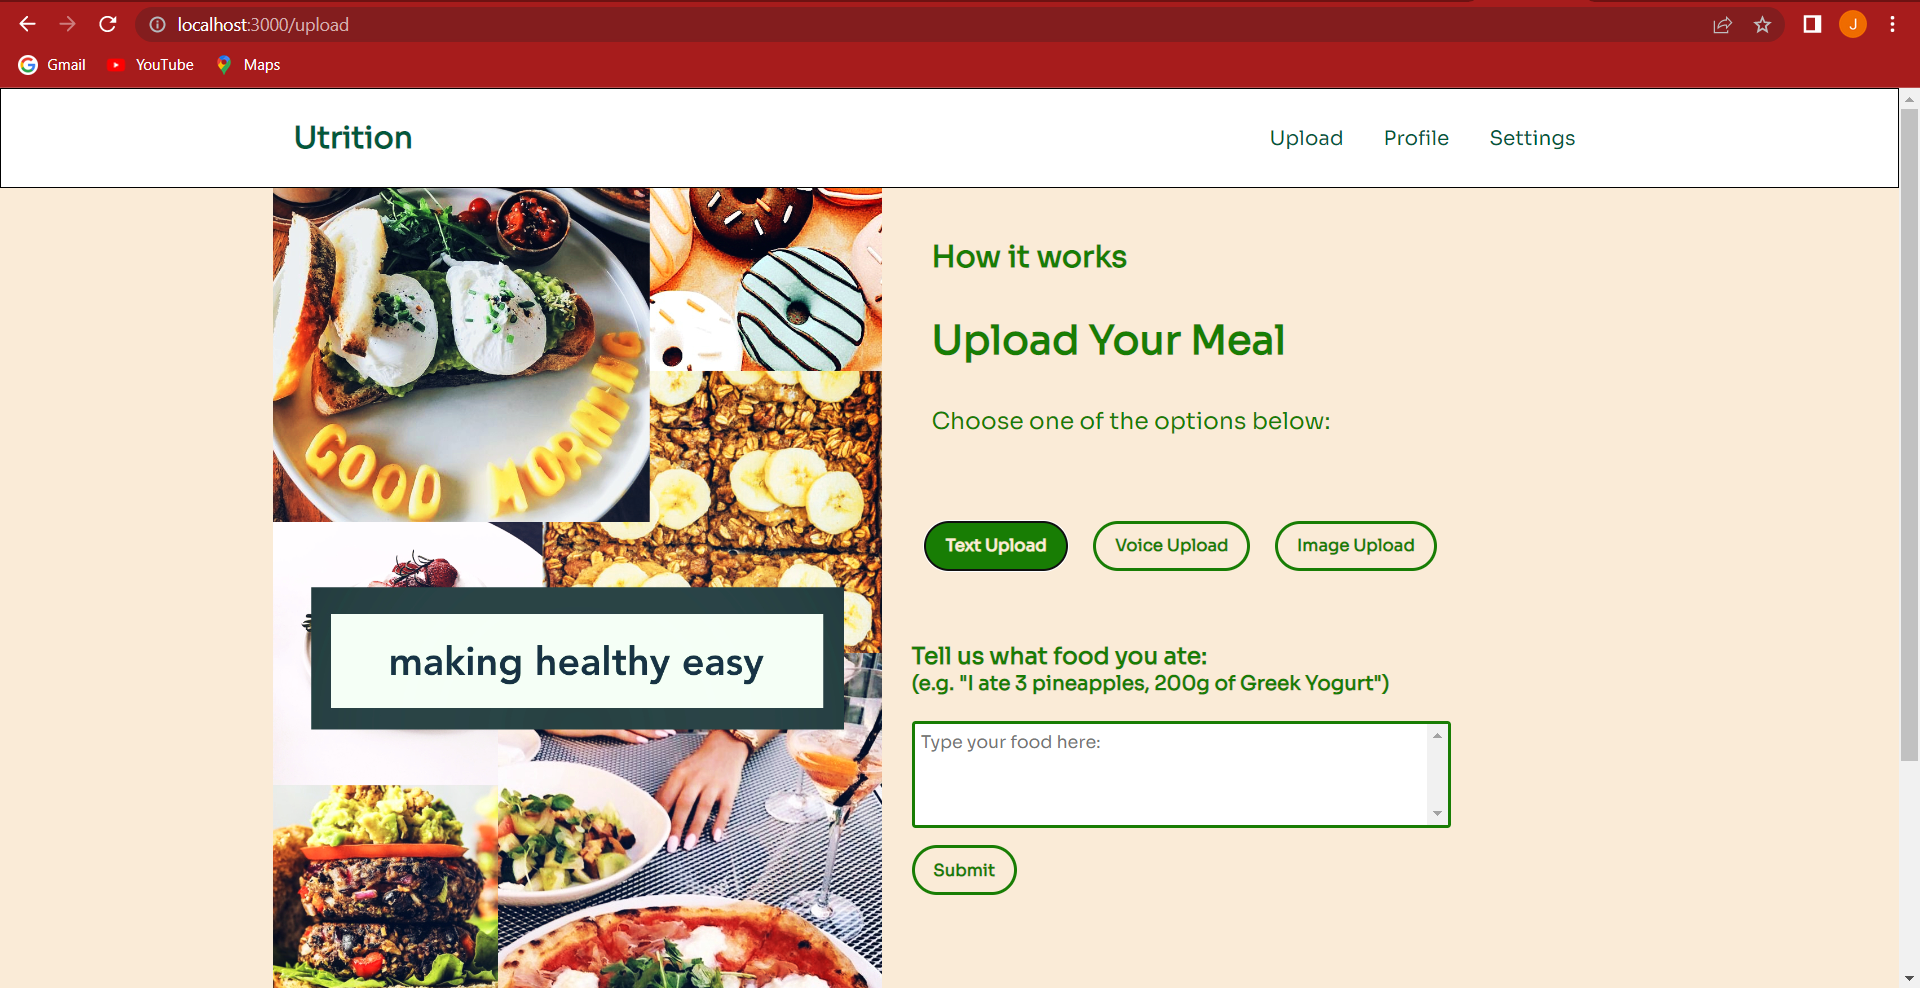
\includegraphics[scale=0.30]{textupload.png}
	\caption{Upload Page with Text Upload Selected}
\end{figure}
Users have the ability to input one or more food items as well as their specific serving sizes. Once the food input has been typed in, the user must press the ``Submit" button. Utrition will display the nutrition facts of the food input to the user and save the entry for the user to view later. Figure 3 shows a sample output.
\begin{figure}[H]
	\centering
	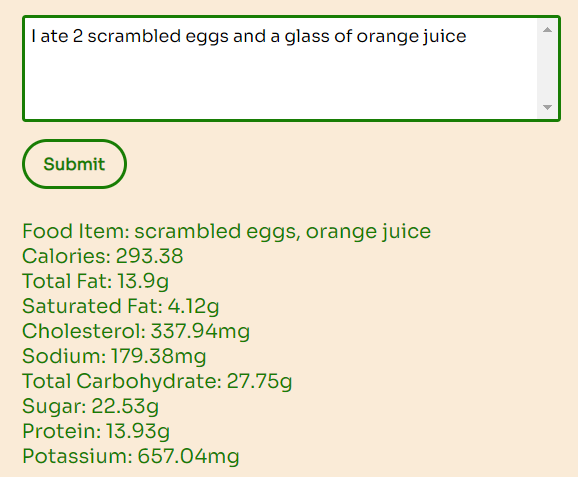
\includegraphics[scale=0.70]{sampleoutput.png}
	\caption{Text output shown by Utrition for sample food input}
\end{figure}

\subsubsection{Voice Upload}
Once on the ``Upload" page, users must select the voice upload button as shown in Figure 4. Buttons will appear where the user can commence audio tracking.
\begin{figure}[H]
	\centering
	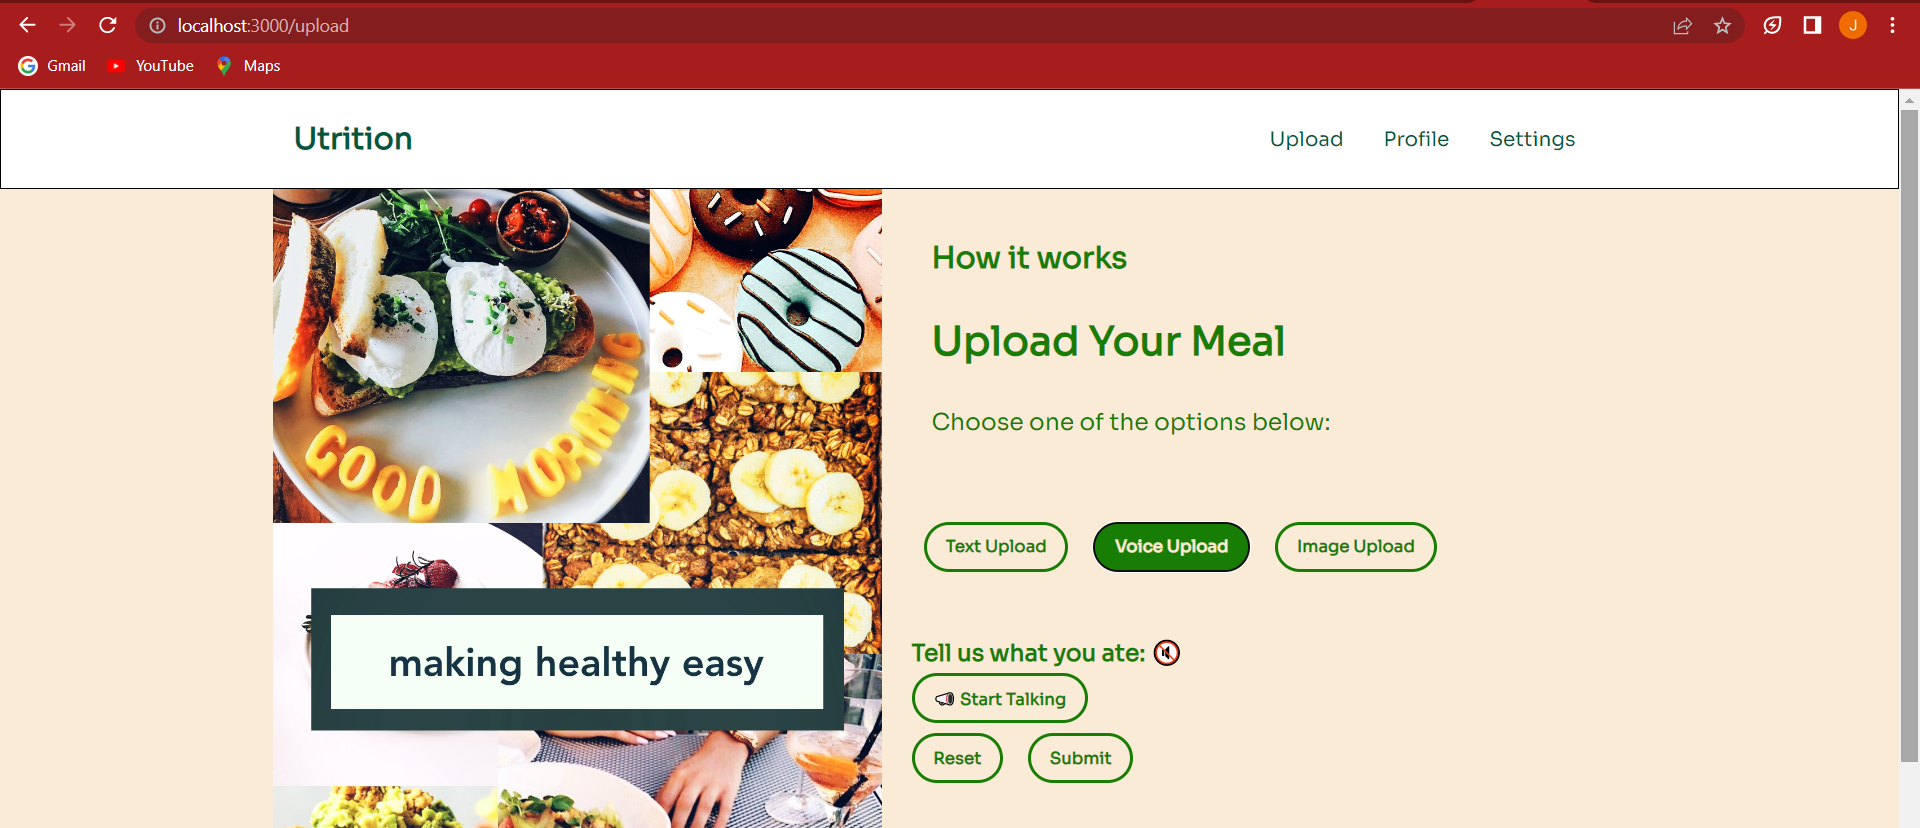
\includegraphics[scale=0.30]{voiceupload.png}
	\caption{Upload Page with Voice Upload Selected}
\end{figure}
Once the user is ready to give their food input, they will click the ``Start Talking" button and begin speaking into the device. Utrition will listen to the user's speech and convert it to text which is displayed to the user. Once finished, the user will click the ``Stop Talking" button and submit their input by pressing ``Submit". If the user wishes to give a different voice input, they can press the ``Reset" button and repeat the explained steps. Similar to text upload, users can input multiple food items and serving sizes at once. A sample output is displayed in Figure 5.

\begin{figure}[H]
	\centering
	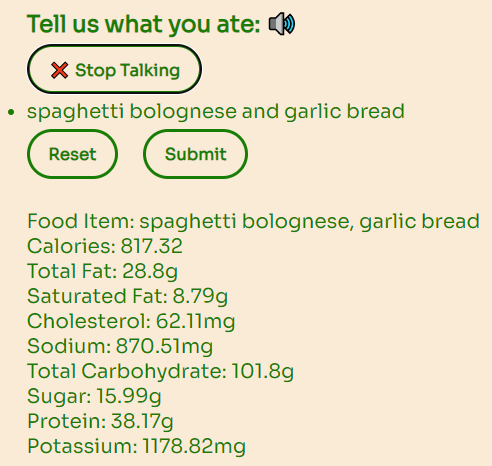
\includegraphics[scale=0.70]{sampleoutputvoice.png}
	\caption{Voice output shown by Utrition for sample food input}
\end{figure}

Once input is submitted, Utrition will display the nutritional information for the specified foods and save the entry for the user to view later.

\subsubsection{Image Upload}
Once on the ``Upload" page, users must select the image upload button as shown in Figure 6. Buttons will appear for the user to select an existing image of a food item from their device.

\begin{figure}[H]
	\centering
	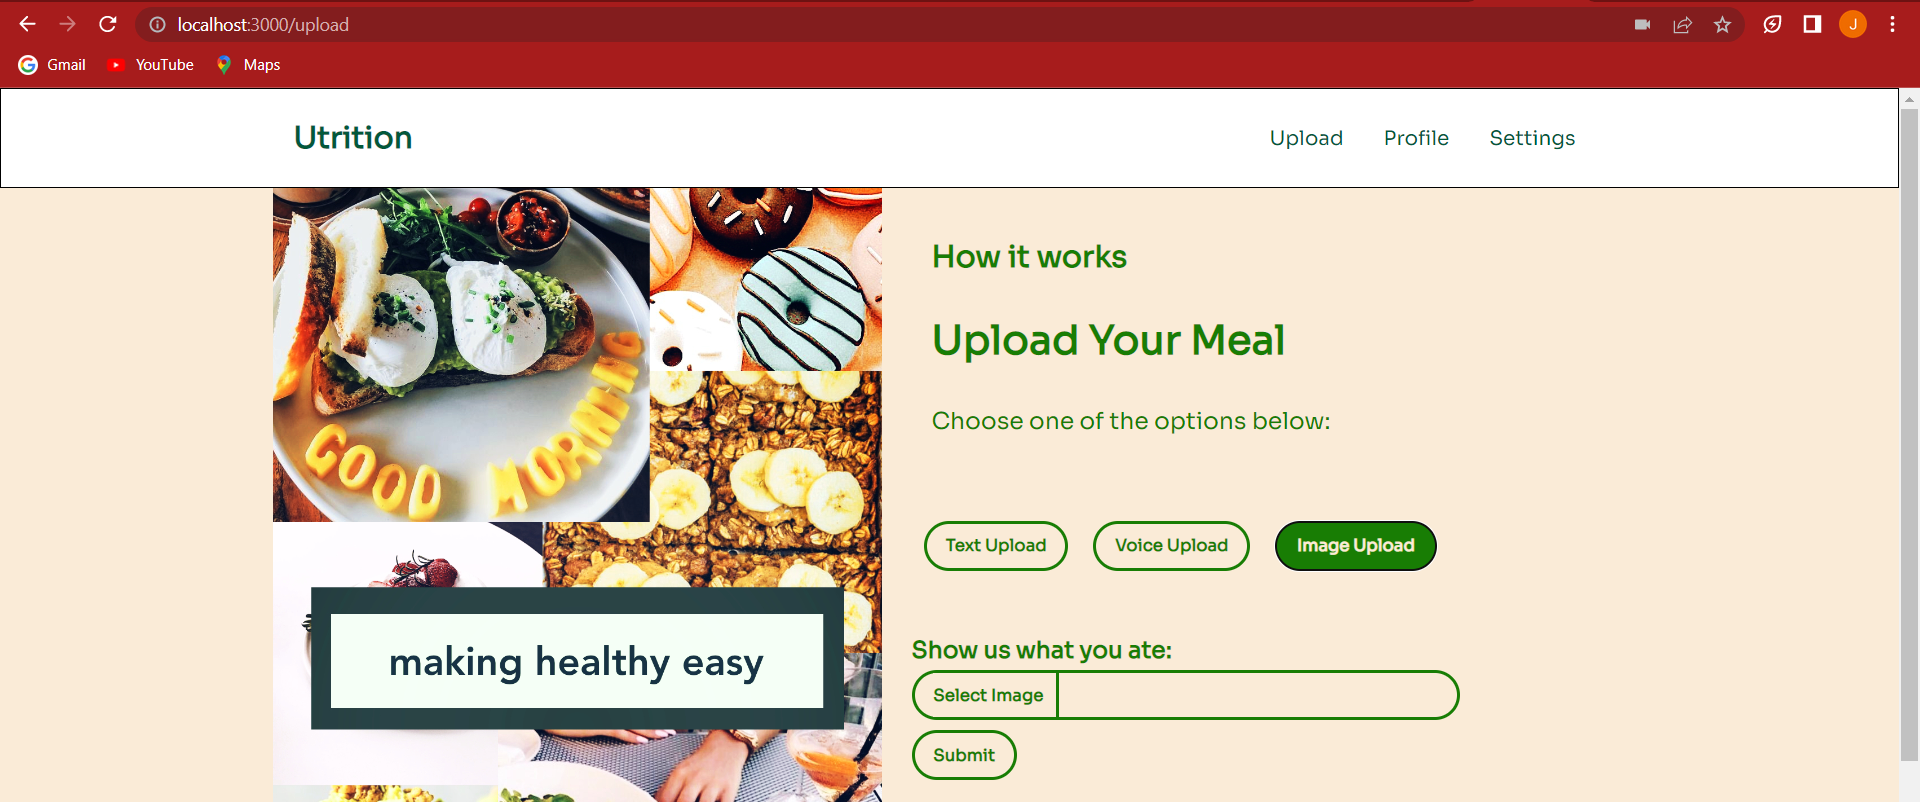
\includegraphics[scale=0.30]{imageupload.png}
	\caption{Upload Page with Image Upload Selected}
\end{figure}

Once the user has selected the food image that they want identified, the user will press the ``Submit" button. Utrition will begin processing the image. Once identified, Utrition will ask the user if its identification of the food item is correct as shown in Figure 7. 

\begin{figure}[H]
	\centering
	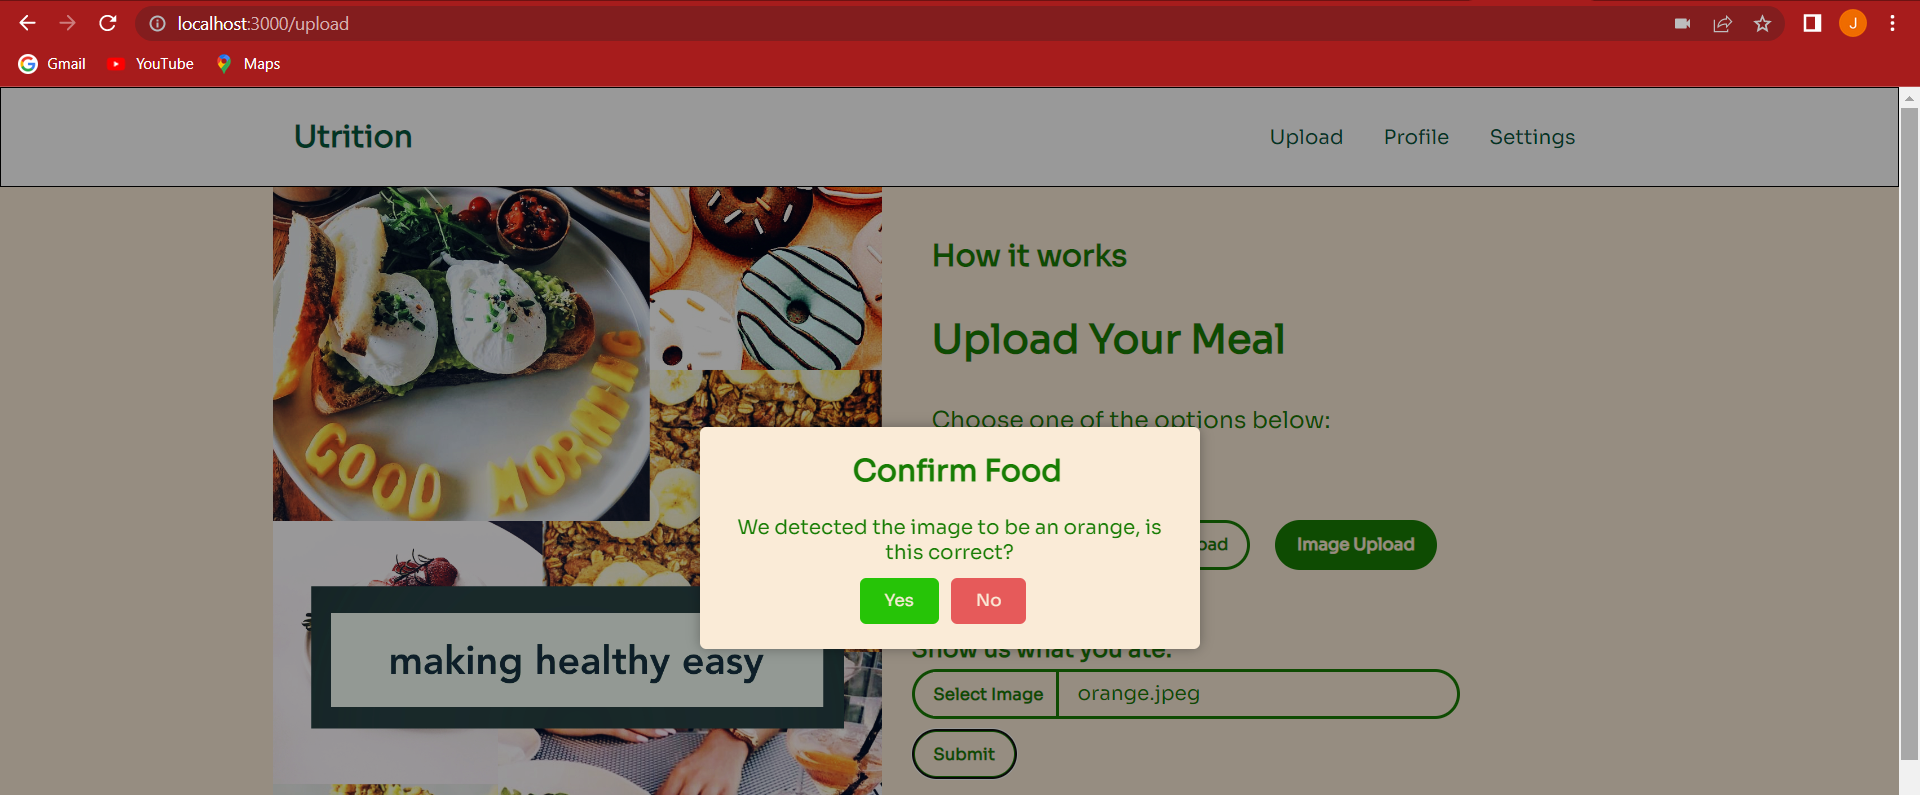
\includegraphics[scale=0.30]{confirmimage.png}
	\caption{Confirmation of identified food}
\end{figure}

If the image is correctly classified, the user will select the ``Yes" button. The interface will then show the nutrition facts of the food input and save the entry for the user to view later as shown in Figure 8. If Utrition did not identify the food correctly, the user will click the ``No" button and will be prompted to upload a new image.

\begin{figure}[H]
	\centering
	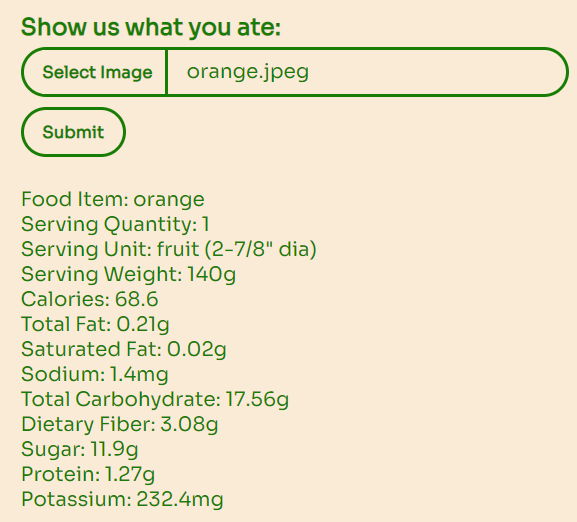
\includegraphics[scale=0.70]{sampleoutputimage.png}
	\caption{Image output shown by Utrition for sample food input}
\end{figure}

\subsection{Viewing Previously Input Foods}
To view previously input food items, the user will navigate to the ``Profile" page. This is done by clicking the ``Profile" text found in the navigation bar at the top of every page. The interface will display an interface similar to that shown in Figure 9.

\begin{figure}[H]
	\centering
	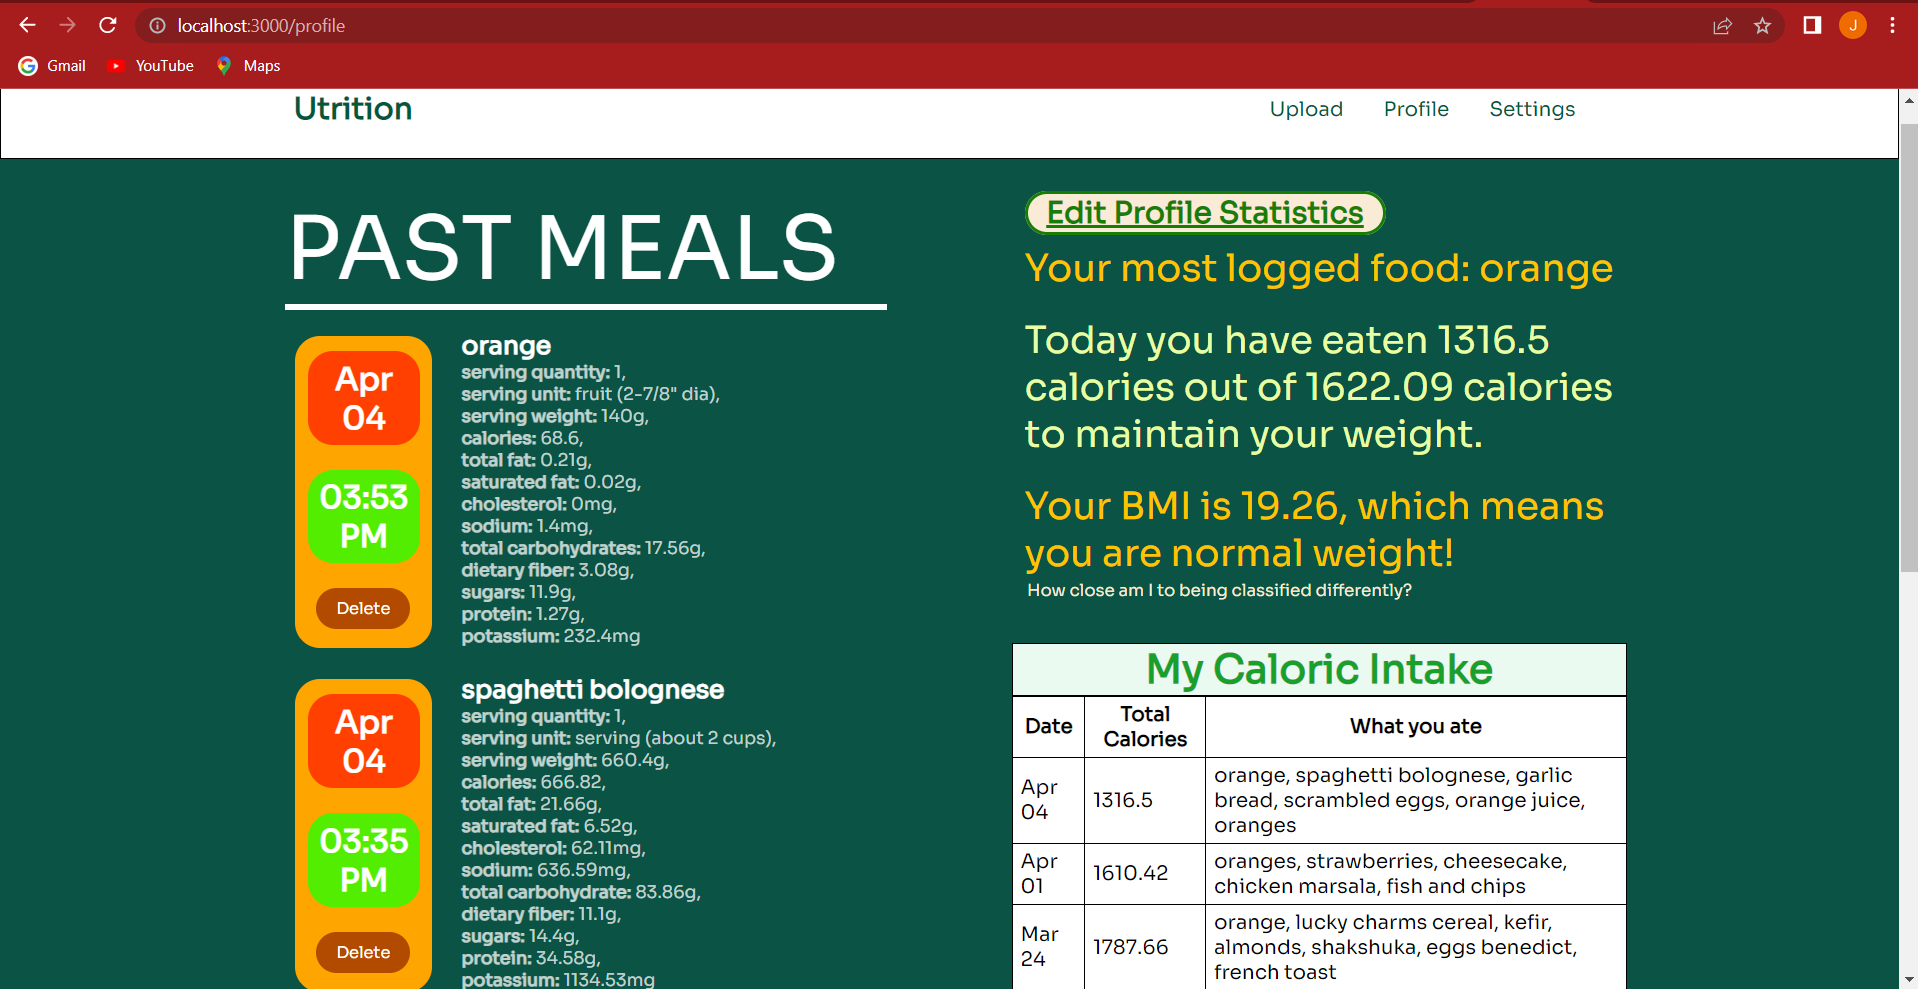
\includegraphics[scale=0.30]{profilepage.png}
	\caption{Sample Profile page}
\end{figure}

This page contains many insights into the user's eating habits. Firstly, every food item inputted by the user and the corresponding nutrition facts are displays under the ``PAST MEALS" header. Food entries are displayed in the order of most recently input. Users can press the left and right arrow buttons at the bottom of the screen to view older entries. On the righthand side of the interface, Utrition displays the user's most eaten food item, their calories for the current day, the recommended calories based on the user's personal statistics, the user's BMI, a caloric summary for each day and a graph displaying the same caloric summary information. A sample graph and caloric summary is shown in Figure 10.

\begin{figure}[H]
	\centering
	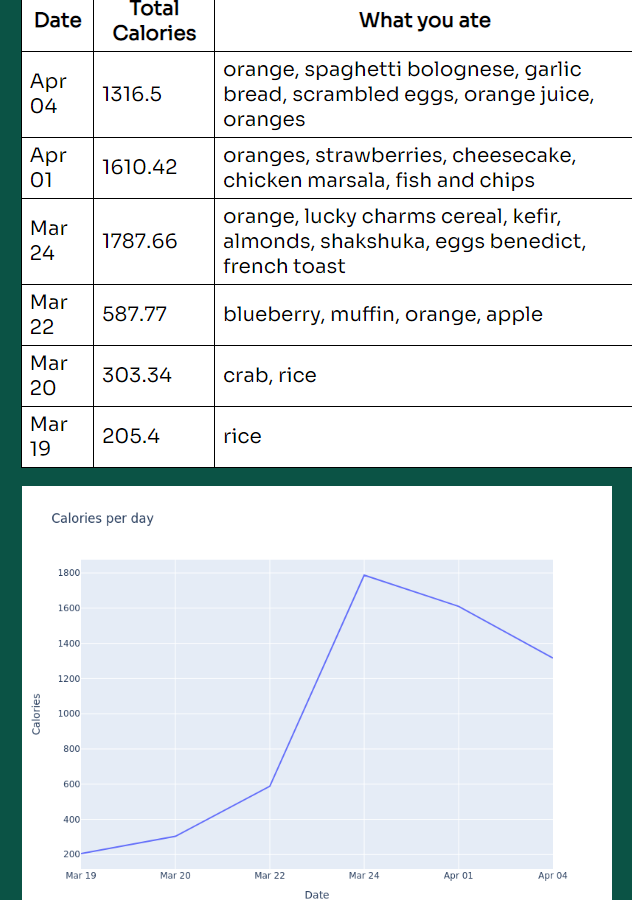
\includegraphics[scale=0.70]{graph.png}
	\caption{Sample graph of caloric intakes}
\end{figure}

\subsection{Deleting a Food Entry}
If a user wishes to delete a previously inputted food item, they must navigate to the ``Profile" page. This is done by clicking the ``Profile" text found in the navigation bar at the top of every page. Once on the page, the user can browse through their previously inputted food items to choose one to delete. The user will click the ``Delete" button on the entry they would like removed. Utrition will prompt the user to confirm that they wish to delete the entry since deletion can not be reversed. This prompt is displayed in Figure 11. If the user selects the ``Yes" button, the food entry will be removed from the user's history.

\begin{figure}[H]
	\centering
	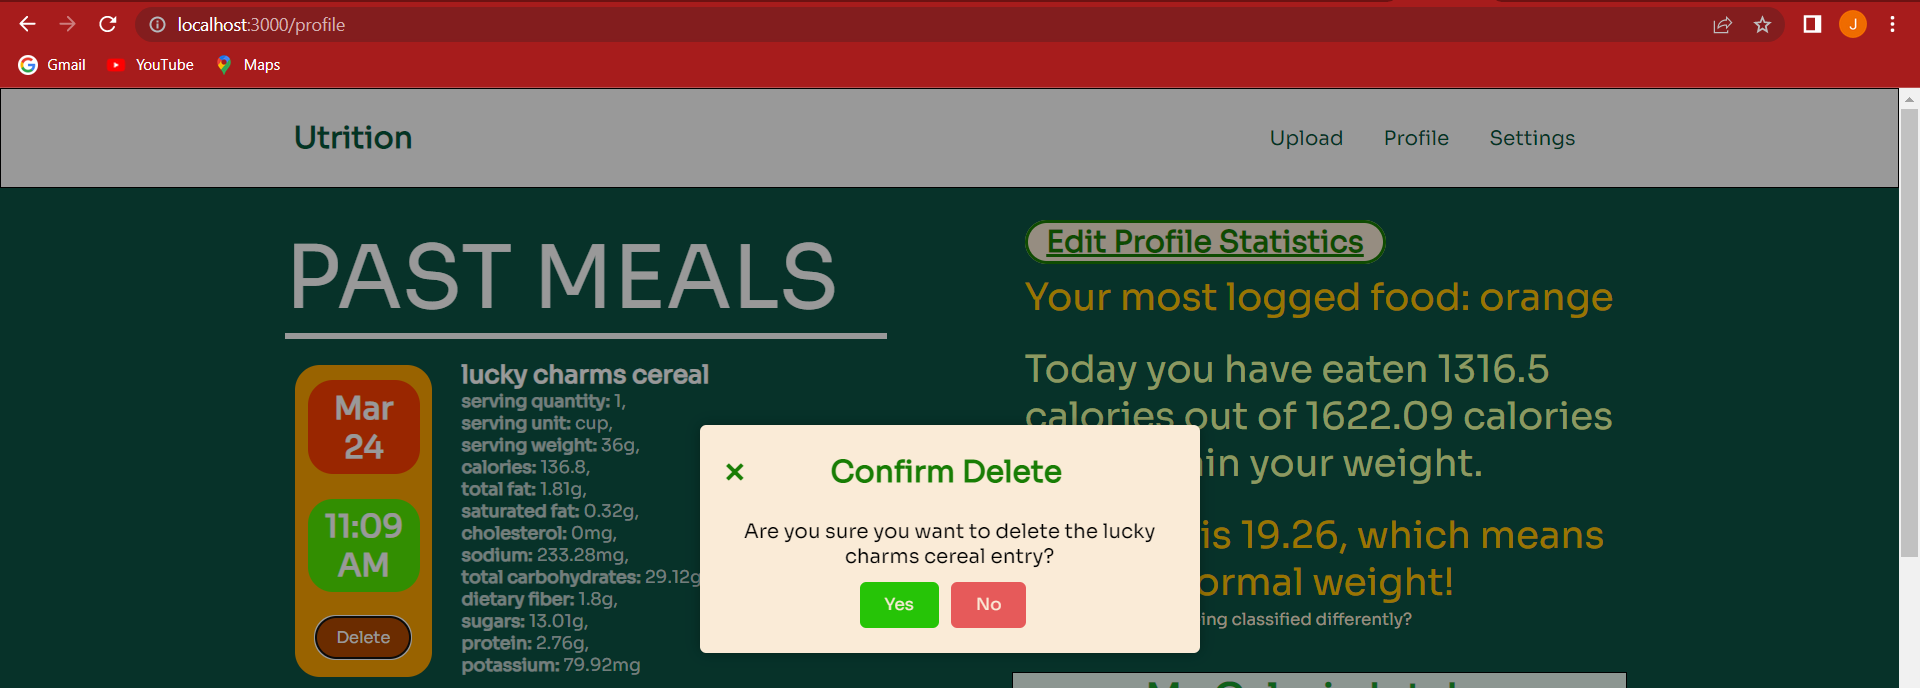
\includegraphics[scale=0.30]{deleteitem.png}
	\caption{Prompt for deleting a food entry}
\end{figure}

\subsection{Editing User Statistics}
Users have the option to input their personal statistics into Utrition. With this information, Utrition will calculate the user's BMI and recommended calories per day. To input user settings, users must navigate to the ``Settings" page. This can be done by clicking on the ``Edit Personal Statistics" button found on the ``Profile" page or by clicking the ``Settings" text found in the navigation bar at the top of every page. Once on the ``Settings" page, the user can see the current user settings that are saved. Figure 12 shows the interface output in the case where no user statistics are saved.

\begin{figure}[H]
	\centering
	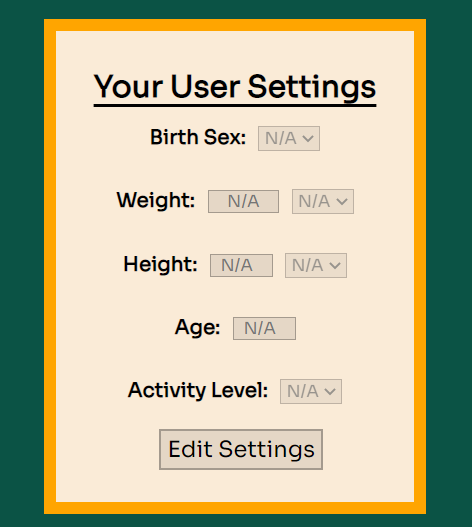
\includegraphics[scale=0.70]{settingspage.png}
	\caption{User settings page with no previously saved statistics}
\end{figure}

Next, users can click the ``Edit Settings" button to input their statistics. This will take them to the interface in Figure 13. On this page, users must fill in the required fields. Weight can be given in pounds or kilograms. Height can be given in feet and inches or centimeters. Once all fields are filled out, the user can save their settings by clicking the ``Save" button. Users can also press the ``Cancel" button to exit out of editing.

\begin{figure}[H]
	\centering
	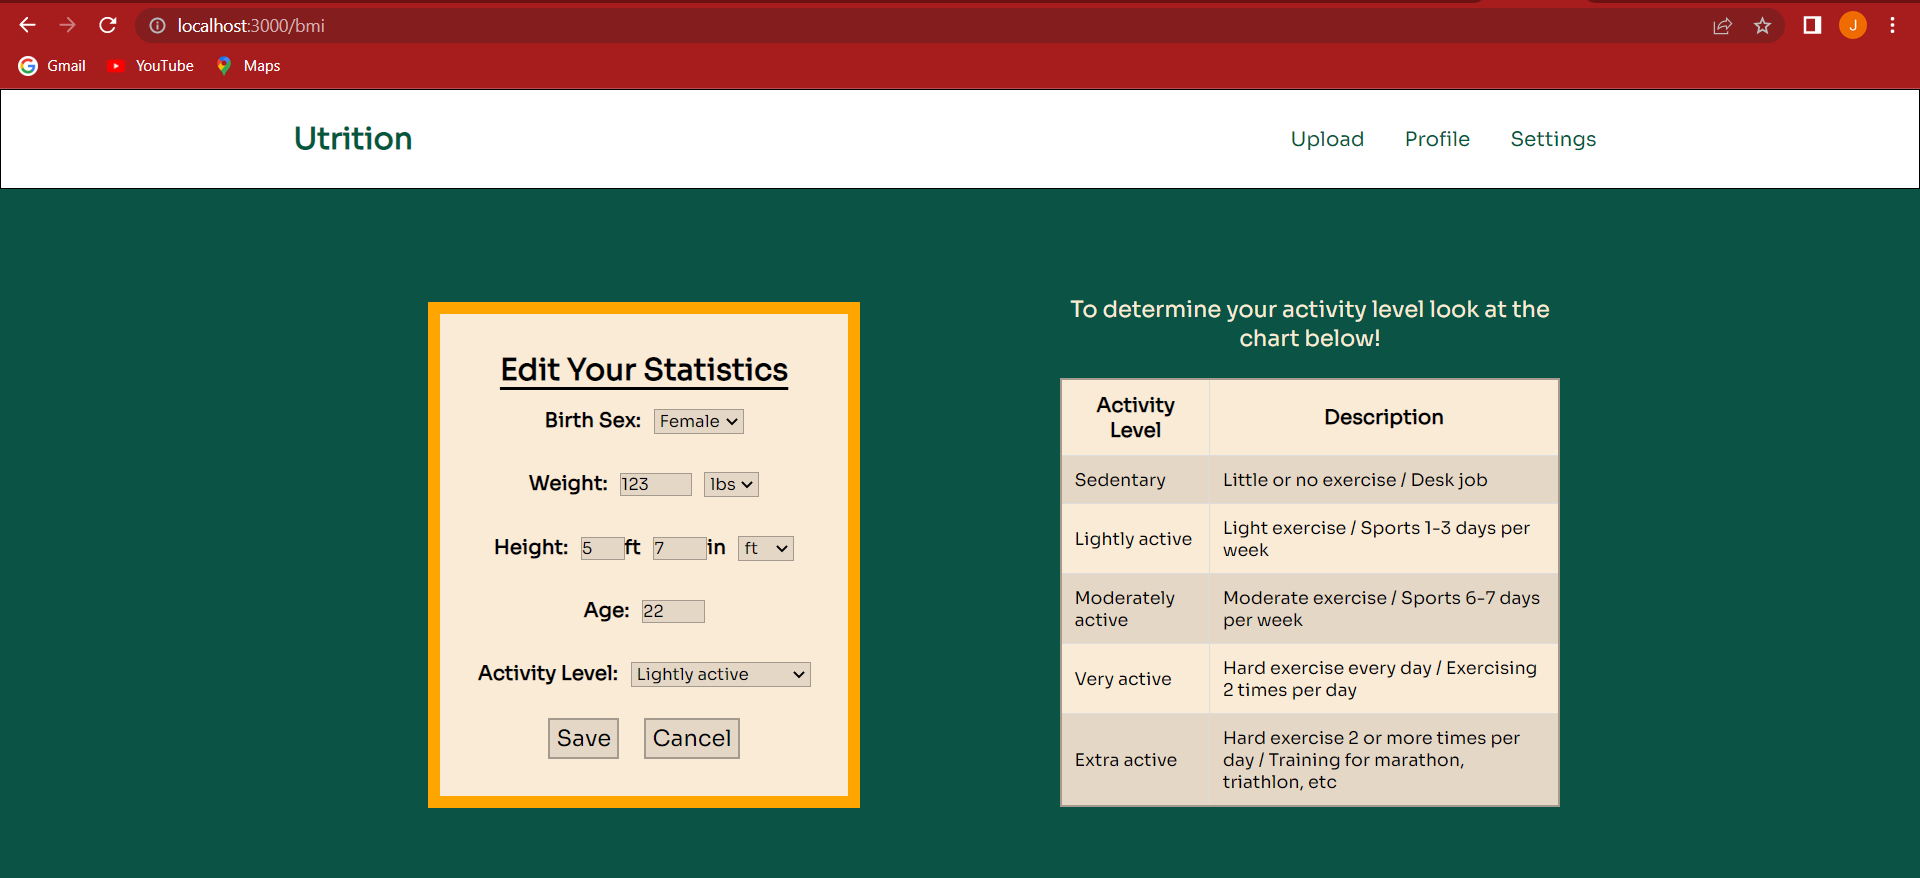
\includegraphics[scale=0.30]{editingsettings.png}
	\caption{Edit Settings Page}
\end{figure}

Once saved, the user will be returned to the ``Settings" page which will now display the user's recently saved statistics (Figure 14). 

\begin{figure}[H]
	\centering
	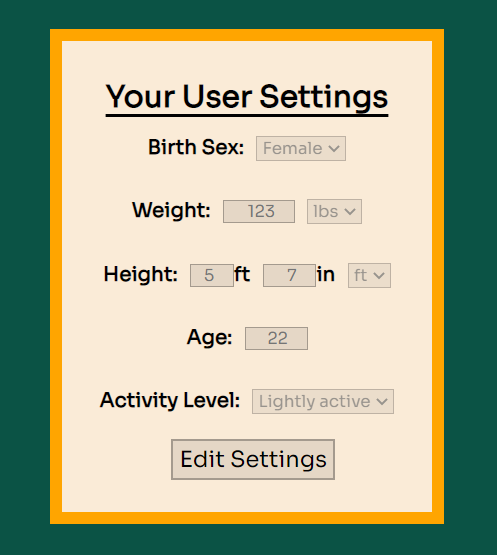
\includegraphics[scale=0.70]{updatedsettings.png}
	\caption{Updated Settings Page}
\end{figure}

\section{Troubleshooting}
The scenarios discussed below are potential issues that users may face while using Utrition. For additional issues not identified, the user should restart Utrition fully. This includes following the steps found in Section 5 and Section 4 respectively.

\subsection{No Past Entries in Profile Page}
If the user navigates to the ``Profile" page and does not see any past food entries, there are a number of possible reasons and solutions. Firstly, the user should check that they ran the command ``npm run start-backend" to successfully start up Utrition. If this has been done, the user should ensure that they have previously inputted food entries in the ``Upload" page. Restarting Utrition should be done if both of these conditions have been satisfied.

\subsection{No Nutritional Data Displayed Upon Input Submission}
While uploading a food input to Utrition, there may be a case where no nutritional data is presented to the user. This will only occur when the user's device is not connected to the internet. To resolve the issue, the user must connect to the internet and resubmit their previous input. 

\section{Frequently Asked Questions}
\subsection{Why can my food image not be classified?}
In some cases, Utrition will be unable to classify a food image correctly even after multiple submissions. Utrition's image classification technology was trained with a small group of foods which most likely does not contain the food in the inputted image. Utrition's developers will improve upon this feature in future code updates. For the time being, users should try inputting their food in text or voice upload to avoid this error.
\subsection{Is my data saved to an online server?}
Utrition is a completely local application. This means that all saved data including personal statistics and past food entries are stored directly on the user's device. Other Utrition users and developers have no way of accessing a user's data.

\end{document}